\section{諸概念}

\subsection{eスポーツ}

eスポーツとは,コンピュータゲームをスポーツとして捉える際の名称である.そのため,特定のゲームを指すものではない.%よって,eスポーツの定義自体一意的に定まっていない.そのためメディアによって様々に定義が異なる.
eスポーツにはジャンルがあり,一般的に大きく分けてMOBA(マルチプレイヤー・オンライン・バトル・エリア),シューター,格闘,パズル,スポーツ,RTS(リアルタイムストラテジー),OCG(オンラインカードゲーム)の7種類と言われている.

\subsection{eスポーツの市場規模}

世界のeスポーツの市場規模は2015年には3億2500万ドルだったのが2020年には11億ドルまで成長すると予想されている.(2020年時点).日本esports促進協会によると,世界のeスポーツ観戦者・視聴者数は2015年には2億3千万人だったが,2023年には6億人を突破するだろうと予想されている.%これはパンデミックに伴うロックダウン施策によってライブストリーミング視聴に多くの時間を費やすユーザーが増加したからとも考えられる.
観戦者・視聴者の増加もあり,eスポーツの市場規模は年々拡大している.

近年,日本でもeスポーツの本格化が始まった.大都市圏では,ゲームメーカーなどが大型のeスポーツイベントを定期的に開催し,大会の様子はライブ配信されている.%コロナ禍により市場規模は成長を鈍化させたが,
日本eスポーツ連合は2018年は推定48億円であり,2024年は150億円になると試算しており,コロナ禍が落ち着けば年平均20%を超える成長率が見込めるとしている.国内大手のゲームメディアであるファミ通は2018年は推定約48億円であり,2024年には約184億円になると予測している.日本のeスポーツは遅れており黎明期だと言われているが,今後の拡大が十分に期待されている分野と言える.

\subsection{eスポーツの歴史}

eスポーツの歴史は1970年代まで遡り,1972年にスタンフォード大学の学生が開催した「Space war」の大会が始まりだと言われている.1974年には「セガTVゲーム機全国コンテスト東京決勝大会」が開催された.1978年に「スペースインベーダー」が発売され,1980年にATARI(アタリ,アメリカのゲーム会社)が「Space Invaders championship」を開催した.この大会には全米で1万人の参加者が集まり,最初の大規模なコンピュータゲーム大会と言われている.

1990年代に日本では対戦型格闘ゲームが人気になった.インターネットの普及がゲームによる対戦,ゲームのスポーツ化に拍車をかけた.それに並行して欧米では1997年にPGL%(Professional Gamers League)
やCPL%(Cyberathlete Professional League)
が設立され,プレイヤーのプロ化が始まった.この頃からeスポーツという言葉が選手や関係者間で認知され始めた.

1995年にBattele by the Bay(後のEVO)%:The Evolution championship Series)
が開催された.2000年にWCGC%(World Cyber Games Challenge)
が開催された.%「eスポーツ」という単語が使われ始める.
2003年に中国国家体育総局が99番目の正式体育種目に指定した.2004年にロシア政府が後援したRussian Cupが開催された.2006年にOCA主催第2回アジア室内競技大会でeスポーツが正式種目に採用することが決定された.%,翌年2007年にマカオで開催された.
2011年に第1回eスポーツJAPAN CUPが開催され,ライブ配信サイトTwitchが立ち上げられた.%ゲーム配信者によるゲーム配信で人気のTwitchだが,eスポーツの大会の様子も配信されている.
YouTube等の動画配信サイトやライブ配信サイトの登場により,eスポーツの市場は急成長を遂げた.

%\documentclass[a5j]{jarticle}
%\usepackage[dvipdfmx]{graphicx}
%\begin{figure}[htbp]
%    \begin[center]
%    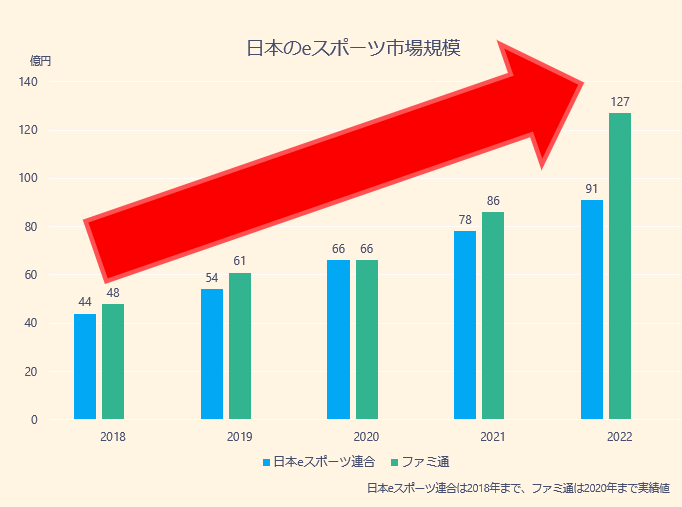
\includegraphics{sijoukibo.png}
%    \caption{市場規模}
%\end{center}
%\end{figure}

\subsection{教育とeスポーツ}

日本の教育現場ではeスポーツに対する印象はあまりよくないのは事実であるが,海外でeスポーツは受け入れられている.ノルウェーの公立高等学校では,選択科目としてeスポーツをサッカーなどの従来のスポーツとして位置づけられている.また,韓国ではeスポーツで優秀な成績を収めた生徒は従来のスポーツ推薦のようにeスポーツ推薦を受け,大学を受けることができる.

日本の教育現場でeスポーツが受け入れられにくい要因について,笹川スポーツ財団「スポーツの歴史」によると,日本人はスポーツと縁が薄く,楽しむことを罪悪のように考え,「スポーツは体を鍛える」とされていることにあると述べている.さらに,日本には古来,身体活動を通して精神を磨くという伝統が色濃く残っていた点にもあると述べている.%座禅を組み,武士道に代表される「道」は,能狂言や茶の湯,生け花といった「楽しみ」に「極める」ことを求めた.
